% vim: set textwidth=78 autoindent:
    
\subsection{Das CSV-Plugin benutzen}\label{label_dltext}    

Mit dem 'CSV'-Plugin\footnote{CSV steht f�r comma-separated-value, also
Textdateien, dessen Spalten mit einem definierten Trennzeichen versehen
sind} k�nnen Datenspalten aus einer Textdatei als ein Layer
in QGIS geladen werden. 
    
\subsubsection{Anforderungen}

Um Datenspalten aus einer Textdatei in QGIS zu laden, muss diese Textdatei
bestimmte Eigenschaften haben:

\begin{enumerate}      
\item Eine Kopfzeile mit den Spaltennamen. Diese Kopfzeile muss die erste Zeile 
der Datei sein   
\item Die Textdatei muss mindestens eine Spalte mit X- und eine mit Y-Koordinaten enthalten. 
Die Bezeichnungen in der Kopfzeile f�r diese Spalten k�nnen beliebig sein.
\item Die X- und Y-Koordinaten m�ssen als Zahlen angegeben sein. Das
Koordinatensystem spielt keine Rolle.
\end{enumerate}

Ein Beispiel f�r einen Textdatei k�nnte so aussehen:

\begin{verbatim} 
name|latdec|longdec|cell|
196 mile creek|61.89806|-150.0775|tyonek d-1 ne|
197 1/2 mile creek|61.89472|-150.09972|tyonek d-1 ne|
a b mountain|59.52889|-135.28333|skagway c-1 sw|
apw dam number 2|60.53|-145.75167|cordova c-5 sw|
apw reservoir|60.53167|-145.75333|cordova c-5 sw|
apw reservoir|60.53|-145.75167|cordova c-5 sw|
aaron creek|56.37861|-131.96556|bradfield canal b-6|
aaron island|58.43778|-134.81944|juneau b-3 ne|
aats bay|55.905|-134.24639|craig d-7|
\end{verbatim}

Einige weitere Anmerkungen zu Textdateien: 

\begin{enumerate}        
\item  Die Beispieldatei verwendet \mbox{$|$} als Trennzeichen. Es k�nnen auch
andere Zeichen zum Trennen der Spalten verwendet werden.
\item Die erste Zeile ist die Kopfzeile. Sie enth�lt die Spaltennamen name, latdec,
longdec und cell
\item Anf�hrungszeichen ({\tt{}"{}}) d�rfen nicht als Trennzeichen benutzt
werden
\item Die X-Koordinaten sind in der Spalte {\em longdec} enthalten
\item Die Y-Koordinaten sind in der Spalte {\em latdec} enthalten
\end{enumerate}

\subsubsection{Das Plugin benutzen}

Um das Plugin zu benutzen, m�ssen Sie QGIS starten und den Plugin Manager
aufrufen, um das Plugin \textsl{Getrennter Text} zu aktivieren:

Starten Sie QGIS, �ffnen Sie den Plugin Manager �ber das Men� {\em
Plugins->Plugin Manager} in der Men�leiste. Der Plugin Manager zeigt
eine Liste vorhandener Plugins. Sie k�nnen Plugins mit der entsprechenden
Checkbox aktivieren und deaktivieren und dann auf den Knopf \textsl{Ok} klicken, 
wie in Kapitel \ref{sec:managing_plugins} beschrieben.

Das ausgew�hlte Plugin erscheint nun in der Werkzeugleiste:
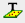
\includegraphics[width=0.7cm]{toolbar_icon}
Klicken Sie auf das Icon, um das Plugin \textsl{Getrennter Text} wie in
Abbildung \ref{fig:delim_text_plugin_dialog} zu starten.

\begin{figure}[ht]
   \begin{center}
   \caption{Getrennter Text Dialog}\label{fig:delim_text_plugin_dialog}\smallskip
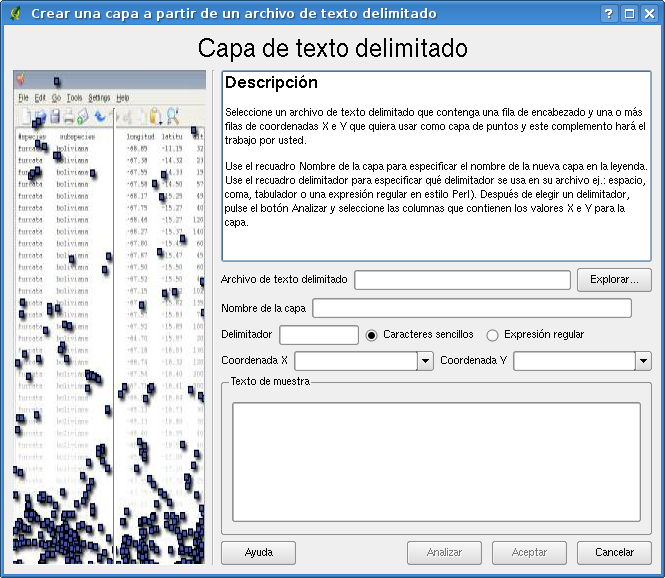
\includegraphics[clip=true, width=8cm]{dialog}            
   \end{center}  
\end{figure}

Zuerst w�hlen Sie eine Textdatei aus, die Sie laden m�chten:
\includegraphics[scale=0.5]{ellipsis}
Das Plugin versucht nun automatisch mit Hilfe des zuletzt verwendeten
Trennzeichens eine Struktur (Spalten) in der Datei zu finden. Im Beispiel ist
es das Trennzeichen \mbox{$|$} (Abbildung \ref{fig:delim_text_file_selected}).
\begin{figure}[ht]
   \begin{center}
   \caption{Ausgew�hlte Textdatei}\label{fig:delim_text_file_selected}\smallskip
\includegraphics[clip=true, width=8cm]{file_selected}   
   \end{center}  
\end{figure}

F�r diese Textdatei ist das Trennzeichen \mbox{$|$} nicht richtig, sie wird
durch TABs getrennt. Beachten Sie, dass die X- und Y-Felder nicht die g�ltigen
Spaltennamen enthalten.

\begin{figure}[ht]
   \begin{center}
   \caption{In der Textdatei gefundene Spalten}\label{fig:delim_text_file_selected2}\smallskip  
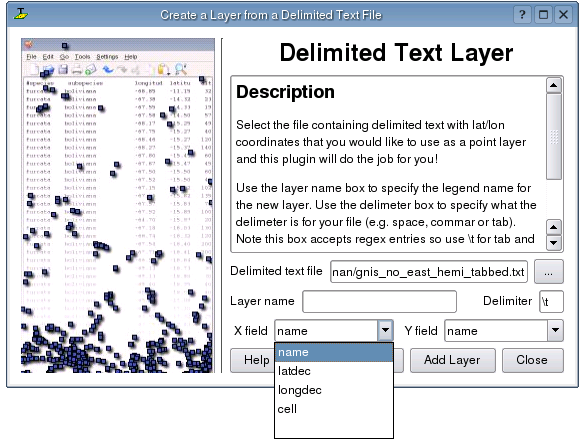
\includegraphics[clip=true, width=8cm]{file_selected2}
   \end{center}  
\end{figure}

Damit die Textdatei richtig durchsucht werden kann, �ndern Sie das Trennzeichen auf \mbox{$\backslash$}t. Dies ist das regul�re Darstellung des Tabulator-Trennzeichens. Nun klicken Sie auf \textsl{durchsuchen}. Im unteren Feld ist der Inhalt nun korrekt in die vorkommenden Spalten unterteilt, wie in Abbildung \ref{fig:delim_text_file_selected2} zu sehen.

\begin{figure}[ht]
   \begin{center}
   \caption{Die X- und Y-Spalten ausw�hlen}\label{fig:delim_text_file_selected3}\smallskip
\includegraphics[clip=true, width=8cm]{file_selected3}
   \end{center}  
\end{figure}

W�hlen Sie nun die Spalten f�r die X- und Y-Koordinaten aus und tragen einen Namen ein, unter dem die Daten in QGIS angezeigt werden sollen (siehe Abbildung \ref{fig:delim_text_file_selected3}. Um die Daten zu sehen, klicken Sie auf \textsl{Hinzuf�gen}. Der Layer verh�lt sich nun wie jeder andere Vektorlayer in QGIS.

 
